\documentclass[11pt,onecolumn]{article}
\usepackage{fancyvrb}
\usepackage{relsize}
\usepackage{fullpage}
\usepackage{amsmath} % for \text; HeVeA doesn't know about amstext
\usepackage{latexsym} % for \Diamond
\usepackage{hevea}
\usepackage{comment}
\usepackage[dvips]{graphicx}       %%% graphics for dvips
\usepackage[colorlinks=true, linkcolor=blue, 
  citecolor=blue, urlcolor=blue,
  ps2pdf,                %%% hyper-references for ps2pdf
  bookmarks=true,        %%% generate bookmarks ...
  bookmarksnumbered=true,%%% ... with numbers
]{hyperref}
% pdfcreator and pdfproducer are set automatically in pdfLaTeX
\hypersetup{ pdfcreator  = {LaTeX with hyperref package},
  pdfproducer = {dvips + ps2pdf} }
\begin{latexonly}
% HeVeA can't handle this:
\let\url\nolinkurl % because dvips cannot break url across lines
\end{latexonly}
%\usepackage{times}

%\includecomment{svn}
%\excludecomment{release}
\includecomment{release}
\excludecomment{svn}

\begin{svn}
\newcommand{\sreither}[2]{#1}
\end{svn}
\begin{release}
\newcommand{\sreither}[2]{#2}
\end{release}

% Make \_ be CMTT's underscore, not \textunderscore, since we use
% it in code and command names.
\def\_{\char"5F}
\newcommand{\todo}[1]{\textbf{[[#1]]}}
\newcommand{\mytt}{\small \tt}

\newcommand{\titled}{Vine installation and user manual}
\title{\mbox{}\\[-.8in]\bf \titled}
\author{BitBlaze Team}
\date{August 26th, 2009:
\sreither{SVN trunk r4183}{Release 1.0}
and Ubuntu 9.04}
\begin{document}
\maketitle

\tableofcontents

\section{Introduction}

This document is a guide for setting up and running Vine, the static
analysis component of the BitBlaze Binary Analysis Framework. It
assumes that you have some familiarity with Linux.  The instructions
are based on
\begin{svn}
the version of Vine in the SVN trunk as of the date shown
in the header,
\end{svn}
\begin{release}
the release of Vine mentioned in the header,
\end{release}
running on a vanilla Ubuntu 9.04 distribution of Linux.
It includes details about how to install Vine, and then walks through
a simple usage example intermixed with explanations about the tools
used.

The example takes a trace from a simple program with symbolic keyboard
input, and generates an STP file which models the weakest precondition
of the control-flow path the program took. In other words, the
conditions on the inputs that cause it to take a execute a certain
path of code. The trace file was generated using TEMU, the dynamic
component of the BitBlaze Binary Analysis Framework, but it is
included in the {\tt examples} directory of the Vine distribution so
you can try out the tool without using TEMU.

\section {\label{sec:install}Installation}

Vine is written using a combination of OCaml and C++, and distributed
in source code form.
%
Therefore the main steps in installing it are installing the
prerequisite software it requires, and then compiling the source code.
%
To install prerequisite software, we recommend that you use a recent
version of Ubuntu Linux, for which we have verified that all the
needed packages are already available.
%
The compilation is performed automatically using {\tt configure} and
{\tt Makefile} scripts like many other Linux applications.
%
The following subsections cover these tasks in more detail, and then
we finish by giving complete listing of the commands needed for our
recommended platform.

\subsection{\label{sec:prereqs}Prerequisites}

Our recommended platform for using Vine is a 32-bit x86 version of
Ubuntu Linux, version 9.04 (code named ``Jaunty Jackalope''); we used
such a system in preparing these instructions.
%
The needed packages all also exist in Debian Linux, so the process
there should work in almost the same way.
%
It is possible to use Vine with other Linux distributions, but you may
need to compile some of the prerequisite software from source.
%
The pure OCaml parts of Vine also work fine on 64-bit x86-64 Linux
platforms, but the library it uses for the semantics of x86
instructions expects to run on a 32-bit platform when processing
32-bit code, so a 32-bit platform is needed to make complete use of
Vine.
%
If you are using an x86-64 version of Ubuntu or Debian, we recommend
installing a parallel 32-bit version of your OS packages using a
mechanism called a ``chroot'', but how to do so is beyond the scope of
this manual (or you could use another kind of virtual machine).

If you don't have any of the prerequisites already installed, they
will require about 300MB to download, and take up about 1.1GB of disk
space once installed.
%
A build of Vine itself requires about 320MB.

\begin{svn}
\subsubsection{Subversion}

Both the development versions of Vine itself and the VEX library we
use are maintained using the Subversion version control system, so
you'll need it to download them. In Ubuntu 9.04, version 1.5.4 is
available in the package {\tt subversion}.
\end{svn}

\begin{svn}
\subsubsection{Autoconf and Automake}

If you are building from the SVN development version of Vine, you will
need to regenerate the {\tt configure} and {\tt Makefile.in} files
needed by the compile using the automake and autoconf tools. In Ubuntu
9.04, you can get suitable versions of both (Automake 1.10.2 and
Autoconf 2.63) by requesting the {\tt automake} package.
\end{svn}

\subsubsection{C++ compiler}

For compiling the C++ code in Vine, we recommend the G++ compiler from
GCC which is standard on Linux; the default version in Ubuntu 9.04 is
4.3.3, and the package name is {\tt g++}.

\subsubsection{\label{sec:vex}The VEX library}

Vine uses the VEX library (which is also used by Valgrind) to get
information about the behavior of x86 instructions.
%
The current version of Vine is designed to work with SVN revision
r1856 of VEX, which is maintained in the Valgrind SVN repository at
\url{svn://svn.valgrind.org/vex/trunk}.
%
\begin{svn}%
You can check it out into a directory named {\tt vex} using the
following command:

\begin{Verbatim}[frame=lines, framesep=.5em]
svn checkout -r1856 svn://svn.valgrind.org/vex/trunk vex
\end{Verbatim}

Then, to compile it, run the following commands in the {\tt vex}
directory:

\begin{Verbatim}[frame=lines, framesep=.5em]
make version
make libvex_x86_linux.a
make libvex.a
\end{Verbatim}
\end{svn}
\begin{release}
For your convenience, we have included an appropriate version of VEX
with the release, and it will be compiled automatically.
\end{release}

\subsubsection{STP}

Vine interfaces with STP, a satisfiability-modulo-theories (SMT)
decision procedure for bit vector (bounded integer) arithmetic and
arrays.
%
Vine can either interact directly with the prover through a
programmatic interface, or it can produce formulas in STP's text
format.
%
The directory {\tt stp} contains x86 and x86-64 binaries for a version
of STP we have tested to work well with Vine.
%
If you would like to use a different version of STP, it is available
in source form at
\url{http://people.csail.mit.edu/vganesh/STP_files/stp.html}.

\subsubsection{Binutils libraries}

Vine uses the GNU BFD (Binary File Descriptor) library and related
libraries from the GNU Binutils to parse the structure of executables,
and for human-readable dissassembly. On Ubuntu they are distributed in
a package named {\tt binutils-dev} (version 2.19.1 in Ubuntu 9.04).

(A technical legal point: the VEX library with which Vine links is
distributed under version 2 of the GNU GPL only, whereas versions 2.18
and later of the GNU Binutils are distributed only under versions 3
and later of the GNU GPL.
%
Unfortunately, versions 2 and 3 of the GPL are mutually incompatible,
so if you plan to distribute copies of Vine for platforms where the
Binutils are not system libraries in the sense of the GPL, you may
wish to use version 2.17 or earlier of the Binutils instead.)

\subsubsection{OCaml build tools}

Most of Vine is implemented in the functional language OCaml, so OCaml
development tools are required.
%
In addition to the standard OCaml compiler and tools, Vine uses the
Findlib library for managing OCaml packages, and the CamlIDL tool for
generating interfaces to C code.
%
In Ubuntu 9.04, these are available as the {\tt ocaml} package
(version 3.10.2), the {\tt ocaml-findlib} package (version 1.2.1), and
the {\tt camlidl} package (version 1.05).
%
Optionally, you can also install the natively compiled versions of the
OCaml build tools (which are somewhat faster) from the
{\tt ocaml-native-compiler} package.

\subsubsection{\label{sec:ocamlgraph}ocamlgraph}

The ocamlgraph library provides graph data structures and algorithms,
which Vine uses to represent control flow graphs.
%
Unfortunately, an interface that Vine uses changed incompatibly in
version 0.99 of the library, so the source code we distribute supports
only version 0.99 and later.
%
In Ubuntu 9.04, it is available as the package {\tt
libocamlgraph-ocaml-dev}.
%
Note, however, that the version of the library packaged in earlier
versions of Ubuntu is not compatible.
%
If a recent version of ocamlgraph is not packaged for your system, you
have several options:
\begin{enumerate}
\item {\bf Compile ocamlgraph from source.}
You can obtain the source for the latest version of ocamlgraph from
\url{http://ocamlgraph.lri.fr/}.
%
Note that it only supports installation in {\tt /usr/lib} or {\tt
/usr/local/lib}.
%
Also, some versions of ocamlgraph have a Makefile bug that causes them
to look for interface files in the wrong location, which can be fixed
by applying the following patch to {\tt Makefile.in}:

\begin{Verbatim}[frame=lines, framesep=.5em]
--- Makefile.in.orig
+++ Makefile.in
@@ -210,7 +210,7 @@
 
 install-findlib: META
 ifdef OCAMLFIND
-	$(OCAMLFIND) install ocamlgraph META *.mli \
+	$(OCAMLFIND) install ocamlgraph META $(LIBDIR)/*.mli \
 		graph$(LIBEXT) graph.cmx graph.cmo graph.cmi $(CMA) $(CMXA)
 endif
\end{Verbatim}

\item {\bf Make a backport package.}
If you would like to have the installation of ocamlgraph managed by
your regular package manager, another option is to build a package
yourself. For instance, a suitable package for Ubunutu 8.04 can be
built and installed using Debian sources, as follows:

\begin{Verbatim}[frame=lines, framesep=.5em]
sudo apt-get install   libocamlgraph-ocaml-dev
sudo apt-get build-dep libocamlgraph-ocaml-dev
sudo apt-get install liblablgtk2-ocaml-dev liblablgtk2-gnome-ocaml-dev \
                     docbook-xsl po4a
sudo apt-get install fakeroot
svn co svn://svn.debian.org/svn/pkg-ocaml-maint/trunk/packages/ocamlgraph \
       -r5983
tar xvzf ocamlgraph/upstream/ocamlgraph_0.99c.orig.tar.gz
mv ocamlgraph/trunk/debian ocamlgraph-0.99c
perl -pi -e 's[ocaml-nox \(>= 3.10.0-9\)] #\
              [ocaml-nox  (>= 3.10.0-8)]' ocamlgraph-0.99c/debian/control
(cd ocamlgraph-0.99c && dpkg-buildpackage -us -uc -rfakeroot)
sudo dpkg -i libocamlgraph-ocaml-dev_0.99c-2_i386.deb
\end{Verbatim}

\item {\bf Patch the Vine source.}
Because Vine does not use the extra functionality introduced in the
new library version, another option is to change the Vine code that
uses the library back to the older interface.
%
This requires four one-line changes in four files under {\tt ocaml},
as in the following patch:

\begin{Verbatim}[frame=lines, framesep=.5em]
Index: ocaml/vine_cfg.mli
===================================================================
--- ocaml/vine_cfg.mli
+++ ocaml/vine_cfg.mli
@@ -299,7 +299,7 @@
 
 module Component :
 sig
-  val scc : G.t -> int * ( G.V.t -> int )
+  val scc : G.t -> G.V.t -> int
   val scc_list : G.t -> G.V.t list list
 end
 
Index: ocaml/vine_cfg.ml
===================================================================
--- ocaml/vine_cfg.ml
+++ ocaml/vine_cfg.ml
@@ -1271,7 +1271,7 @@
     if cfg#has_edge rb ra then false
     else (cfg#add_edge rb ra; true) (* temporary backedge *)
   in
-  let (_,scc) = Component.scc cfg in
+  let scc = Component.scc cfg in
   let group = scc a in
   let newcfg = new cfg 8 cfg#get_iter_labels_function cfg#vardecls in
   let (outside: 'a bb) =
Index: ocaml/vine_callstring.ml
===================================================================
--- ocaml/vine_callstring.ml
+++ ocaml/vine_callstring.ml
@@ -178,7 +178,7 @@
   else 
     csg.graph 
   in 
-  let (_,scc) = Component.scc g in 
+  let scc = Component.scc g in 
   let group = scc a in 
   let addifgroup v newg = 
     if scc v = group then
Index: utils/chop.ml
===================================================================
--- utils/chop.ml
+++ utils/chop.ml
@@ -243,7 +243,7 @@
       fun () -> cfg#remove_edge t s 
     ) 
   in
-  let (_,scc) = Component.scc cfg in
+  let scc = Component.scc cfg in
     (* make sure we really have a cycle *)
   let () = assert(scc (cfg#get_id s) = scc (cfg#get_id t)) in 
   let group = scc (cfg#get_id s) in
\end{Verbatim}
\end{enumerate}

\subsubsection{Other OCaml libraries}

Vine also uses several further OCaml libraries:
\begin{itemize}
\item ExtLib provides an extended standard library (e.g., more data
  structures) for OCaml; version 1.5.1 is in the package {\tt
    libextlib-ocaml-dev}.
\item GDome2 is a document object model for dealing with XML documents
  that Vine uses via its OCaml bindings. Version 0.2.6 is available as
  the package {\tt libgdome2-ocaml-dev}.
\end{itemize}

\begin{svn}
\subsubsection{SQLite and its OCaml bindings}

Vine uses the lightweight (serverless) SQL library SQLite, via an
OCaml binding, to store databases of disassembled code with its IDA Pro
static disassembler plug-in.
%
On Ubuntu 9.04, you should install the library itself (version 3.6.10)
via the package {\tt libsqlite3-0} and the OCaml interface via the
{\tt libsqlite3-ocaml-dev} package.
%
It is also convenient to install the command-line database tool, in
the {\tt sqlite3} package.
\end{svn}

\subsubsection{\LaTeX}

Vine's documentation (including this document) is written using the
\LaTeX\ markup language, so you will need to install it to rebuild the
documentation.
%
On Ubuntu 9.04, the needed parts are included under the {\tt texlive},
{\tt texlive-latex-extra}, and {\tt transfig} packages.
%
To build an HTML version of the documentation, we also use \hevea,
which is in the {\tt hevea} package.

\subsection{Compiling}

\begin{svn}
\subsubsection{SVN checkout}

The primary development version of Vine is referred to as the
``trunk'' in the context of our Subversion repository, and it's kept
at the URL \url{https://bullseye.cs.berkeley.edu/svn/vine/trunk}.
%
Note that this repository is password-protected; if someone has
pointed you at this version of these instructions, you should already
have an appropriate account; if you don't, you'll need to get one.
%
For instance, you can check out a copy of the source code into a
directory named {\tt vine} by using the command:

\begin{Verbatim}[frame=lines, framesep=.5em]
svn checkout https://bullseye.cs.berkeley.edu/svn/vine/trunk vine
\end{Verbatim}

\subsubsection{Autoconf and Automake}

To avoid redundancy in the repository, it doesn't store a copy of the
{\tt configure} script or related files, so you will need to
regenerate them by running the {\tt autogen.sh} script; it doesn't
require any arguments.
\end{svn}

\begin{release}
\subsubsection{Unpacking}

Vine is distributed as a gzip-compressed tar archive, which you can
unpack into a directory {\tt vine-1.0} using the command ``{\tt tar xvzf
vine-1.0.tar.gz}''.

\end{release}

\subsubsection{Configure}

To prepare the Vine source for compilation, you'll need to run the
{\tt configure} script in the Vine source directory.
%
The script accepts all of the standard options and environment
variables for autoconf-based configure scripts, though most should not
be necessary.
\begin{svn}
One important option is {\tt --with-vex=}, which you should provide
with the path to the VEX source directory you compiled as described in
section~\ref{sec:vex}.
\end{svn}

\subsubsection{Build code}

After the configuration script has finished, you can compile Vine by
running {\tt make} in the top-level Vine directory.
%
This will compile first the C++ library and then the OCaml modules.

\subsubsection{Build documentation}

To generate the documentation that comes with Vine, go to the {\tt
  vine/doc} subdirectory and give the command ``{\tt make doc}''.

\subsection{Summary}

To recap the steps described above, we now show a script for all of
the commands needed to compile Vine, starting with a fresh
installation of Ubuntu 9.04.
\begin{svn}
(This is also found as the file
\verb'docs/install-vine-svn.sh' in the Vine source.)

\VerbatimInput{../install-vine-svn.sh}
\end{svn}
\begin{release}
(This is also found as the file
\verb'docs/install-vine-release.sh' in the Vine source.)

\VerbatimInput{../install-vine-release.sh}
\end{release}

\section{Vine Overview}

\begin{figure}
\centering
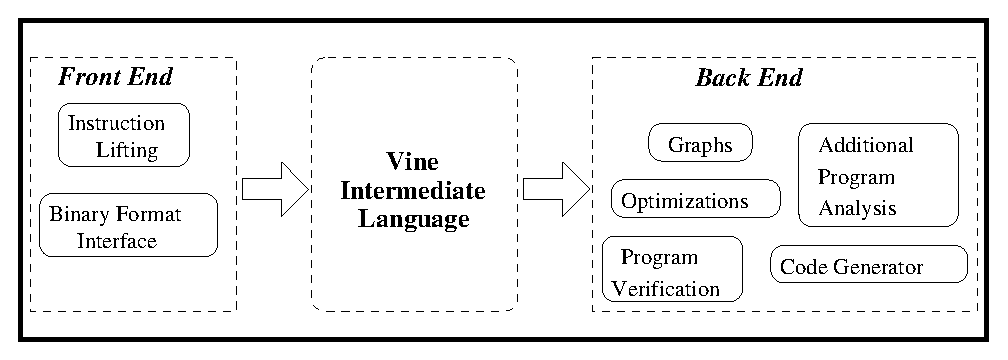
\includegraphics[width=.6\textwidth]{vine-components}
\caption{Vine Overview}
\label{fig:vine-components}
\end{figure}

Figure~\ref{fig:vine-components} shows a high-level picture of
Vine. The Vine static analysis component is divided into a
platform-specific front-end and a platform-independent back-end.  At
the core of Vine is a platform-independent intermediate language
(IL) for assembly.
Previously, we also used the name IR (intermediate representation)
for this language, and that abbreviation persists in some command and
option names, and as a file extension.
The IL is designed as a small and carefully
specified language that faithfully represents the assembly
languages. Assembly instructions in the underlying architecture are
translated to the Vine IL, a process we refer to as {\em lifting}, via
the Vine front-end.  All back-end
analyses are performed on the platform-independent IL. Thus, program
analyses can be written in an architecture-independent fashion and
do not need to directly deal with the complexity of an instruction
set such as x86. This design also provides extensibility---users can
easily write their own analysis on the IL by building on top of the
core utilities provided in Vine.

The Vine front-end currently supports translating 32-bit x86
to the IL. It uses a set of
third-party libraries to parse different binary formats and
produce assembly. The assembly is then translated into the Vine IL in
a syntax-directed manner.

The Vine back-end supports a variety of core program analysis
utilities.  The back-end has utilities for creating a variety of
different graphs, such as control flow and program dependence graphs.
The back-end also provides an optimization framework. The optimization
framework is usually used to simplify a specific set of
instructions. We also provide program verification capabilities such
as symbolic execution, calculating weakest preconditions, and
interfacing with decision procedures.  Vine can also write out lifted
Vine instructions as valid C code via the code generator back-end.

To combine static and dynamic analysis, we also provide an interface
for Vine to read an execution trace generated by a dynamic analysis
component such as TEMU. The execution trace can be lifted to the IL
for various further analysis.


\section{The Vine Intermediate Language}
\label{sec:vine-language}

% Non-terminals from a grammar, suitable for use in math mode.
\newcommand{\nt}[1]{\text{\em #1}}

% Terminals from a grammar, suitable for use in math mode.
\newcommand{\term}[1]{\text{\tt #1}}

\begin{table}
\centering
\begin{footnotesize}
\begin{tabular}{lll}
  \nt{program}&::=&
        \nt{decl}* \nt{stmt}*\\

  \nt{decl}&::=& 
         \term{var} \nt{var}\term{;}\\

  \nt{stmt}&::=&  
         \nt{lval} \term{=} \nt{exp}\term{;}
     $|$ \term{jmp}\term{(}\nt{exp}\term{)}\term{;}
     $|$ \term{cjmp}\term{(}\nt{exp}\term{,} \nt{exp}\term{,} \nt{exp}\term{);}
     $|$ \term{halt}\term{(}\nt{exp}\term{)}\term{;}
     $|$ \term{assert}\term{(}\nt{exp}\term{)}\term{;}\\
     & &  $|$ \term{label} \nt{label}\term{:}
     $|$ \term{special} \nt{string}\term{;}
     $|$ \term{\char"7B} \nt{decl}* \nt{stmt}*\term{\char"7D}\\

  \nt{label}&::=&
         \nt{identifier}\\

  \nt{lval}&::=&
         \nt{var}
     $|$ \nt{var}\term{[}\nt{exp}\term{]}\\

  \nt{exp}&::=&
         \term{(} \nt{exp} \term{)}
     $|$ \nt{lval}
     $|$ \term{name}\term{(}\nt{label}\term{)}
     $|$ \nt{exp} $\Diamond_b$ \nt{exp} 
     $|$ $\Diamond_u$ \nt{exp}
     $|$ \nt{const}\\
     & &  $|$ \term{let} \nt{lval} \term{=} \nt{exp} \term{in} \nt{exp}
     $|$ \term{cast}\term{(}\nt{exp}\term{)}\nt{cast{\tt \_}kind}\term{:}$\tau_{\text{reg}}$\\

  \nt{cast{\tt \_}kind}&::=&  
         \term{Unsigned} $|$ \term{U}
     $|$ \term{Signed} $|$ \term{S}
     $|$ \term{High} $|$ \term{H}
     $|$ \term{Low} $|$ \term{L}\\

  \nt{var}&::=& 
         \nt{identifier}\term{:}$\tau$\\


  $\Diamond_b$&::=&
         \term{+} $|$ \term{-} $|$ \term{*}
     $|$ \term{/} $|$ \term{/\$} $|$ \term{\%} $|$ \term{\%\$}
     $|$ \term{<<} $|$ \term{>>} $|$ \term{\char"40 >>}
     $|$ \term{\&} $|$ \term{\char"5E} $|$ \term{|} \\
     & & $|$ \term{==} $|$ \term{<>}
     $|$ \term{<} $|$ \term{<=} $|$ \term{>} $|$ \term{>=}
     $|$ \term{<\$} $|$ \term{<=\$} $|$ \term{>\$} $|$ \term{>=\$}\\

  $\Diamond_u$&::=& \term{-} $|$ \term{!}\\

  \nt{const}&::=& \nt{integer}:$\tau_{\text{reg}}$ \\

  \nt{$\tau$} &::=&
          \nt{$\tau_{\text{reg}}$} 
      $|$ \nt{$\tau_{\text{mem}}$}\\
  
  \nt{$\tau_{\text{reg}}$}&::=&
          \term{reg1\_t} 
      $|$ \term{reg8\_t} 
      $|$ \term{reg16\_t} 
      $|$ \term{reg32\_t} 
      $|$ \term{reg64\_t}\\

  \nt{$\tau_{\text{mem}}$}&::=& 
          \term{mem32l\_t}
      $|$ \term{mem64l\_t}
      $|$ \nt{$\tau_{\text{reg}}$}\term{[}\nt{const}\term{]}\\
\end{tabular}
\end{footnotesize}
\caption{The grammar of the Vine Intermediate Language (IL).}
\label{vine:syntax}
\end{table}

The Vine IL
is the target language during lifting, as well as the analysis
language for back-end program analysis.  The semantics of the IL are designed
to be faithful to assembly languages.  Table~\ref{vine:syntax} shows
the syntax of Vine IL. 
The lexical syntax of identifiers and strings are as in C.
Integers may be specified in decimal, or in hexadecimal with a prefix
of {\tt 0x}.
Comments may be introduced with {\tt //}, terminated by the end of a
line, or with {\tt /*}, terminated by {\tt */}.

The base types in the Vine IL are 1, 8, 16, 32, and 64-bit-wide bit
vectors, also called registers.
1-bit registers are used as booleans; {\tt false} and {\tt true} are
allowed as syntactic sugar for {\tt 0:reg1\_t} and {\tt 1:reg1\_t}
respectively.
There are also two kinds of aggregate types, which we call {\em arrays}
and {\em memories}.
Both are usually used to represent the memory of a machine, but at
different abstraction levels.
An array consists of distinct elements of a fixed register type,
accessed at consecutive indices ranging from 0 up to one less than
their declared size.
By contrast, memory indices are always byte offsets, but memories may
be read or written with any type between 8 and 64 bits.
Accesses larger than a byte use a sequence of consecutive bytes, so
accesses at nearby addresses might partially overlap, and it is
observable whether the memory is little-endian (storing the least
significant byte at the lowest address) or big-endian (storing
the most significant byte at the lowest address).
Generally, memories more concisely represent the semantics of
instructions, but arrays are easier to analyze, so Vine analyses will
convert memories into arrays, a process we sometimes call {\em
de-endianization}.
The current version of Vine supports two little-endian memory types,
with either 32-bit or 64-bit address sizes.

Expressions in Vine are side-effect free.
Variables and constants must be labeled with their type (separated
with a colon) whenever they appear.
The binary and unary operators are similar to those of C, with the
following differences:
\begin{itemize}
\item Not-equal-to is {\tt <>}, rather than {\tt !=}.
\item The division, modulus, right shift, and ordered comparison
  operators are explicitly marked for signedness: the unadorned
  versions are always unsigned, while the signed variants are suffixed
  with a {\tt \$} (for ``signed''), or in the case of right shift
  prefixed with an {\tt\char"40} (for ``arithmetic'').
\item There is no distinction between logical and bitwise
  operators, so {\tt \&} also serves for {\tt \&\&}, {\tt |} also
  serves for {\tt ||}, and {\tt !} also serves for {\tt \char"7E}.
\end{itemize}
There is no implicit conversion between types of different widths;
instead, all conversions are through an explicit cast operator that
specifies the target type.
Widening casts are either {\tt Unsigned} (zero-extending) or {\tt
Signed} (sign-extending), while narrowing casts can select either the
{\tt High} or {\tt Low} portion of the larger value.
(For brevity, these are usually abbreviated by their first letters.)
A {\tt let} expression, as in functional languages, allows the
introduction of a temporary variable.

A program in Vine is a sequence of variable declarations, followed by
a sequence of statements; block structure is supported with curly
braces.
(In fact, the parser allows declarations to be intermixed with
statements, but the effect is as if the declarations had all appeared
first.)
Some documents also refer to statements as ``instructions,'' but note
that more complex machine instructions translate into several Vine
statements.
The most frequent kind of statement is an assignment to a variable or
to a location in an array or memory variable.
Control flow is unstructured, as in assembly language: program
locations are specified with labels, and there are unconditional ({\tt
jmp}) and conditional ({\tt cjmp}) jumps.
The argument to {\tt jmp} and the second and third arguments to {\tt
cjmp} may be either labels (introduced by {\tt name}), or a register
expression to represent a computed jump.
The first argument to {\tt cjmp} is a {\tt reg1\_t} that selects the
second (for 1) or third (for 0) argument as the target.

A program can halt normally
at any time by issuing the {\tt halt} statement.  We also provide {\tt
  assert}, which acts similar to a C assert: the asserted expression
must be true, else the machine halts.
A {\tt special} in Vine corresponds to a call to an externally
defined procedure or function.  The argument of a special indexes what kind
of special, e.g., what system call.  The semantics of {\tt special} is
up to the analysis; its operational semantics are not defined.  We
include {\tt special} as an instruction type to explicitly distinguish
when such calls may occur that alter the soundness of an analysis. A
typical approach to dealing with {\tt special} is to replace {\tt
special} with an analysis-specific summary written in the
Vine IL that is appropriate for the analysis.



\section{Example}

We now illustrate the use of Vine with an example.
%
In it, we will take a trace generated by TEMU from a program that
parses an integer and checks whether it is equal to 5.
%
We will use Vine to build a version of the execution path in which the
input is symbolic, and compute a path condition: a formula over the
inputs which, if true, causes execution to take the same path.
%
Finally, we will use STP to solve the path condition and reconstruct
an input that would cause the program to take the same path.
%
The trace is included in the {\tt examples} directory under the name
{\tt five.trace}.

\subsection {Generating the IL and the STP formula}

We start with a trace (generated, for instance, by TEMU) that records
the instructions executed on a program run, the data values they
operated on, and which data values were derived from a distinguished
set of (``tainted'') input values. We're going to do operations where
we consider that input to be a symbolic variable, but the first step
is to interpret the trace. The x86 instructions in the trace are a
pretty obscure representation of what is actually happening in the
program, so we'll translate them into a cleaner intermediate language
(IL, abbreviated IR in command options).

First, let us check if we have got a meaningful trace.  One way to do
so is to print the trace, and see that at least the expected
instructions are marked as tainted.  For this, you may use the
\texttt{trace\_reader} command utility in Vine. As shown below, in the
output you should be able to see the compare instruction
that comapares the input to the immediate value 5. The presence of
tainted operands in any instruction are indicated by the record
containing ``T1''.

\begin{Verbatim}[frame=lines, framesep=.5em]

% cd bitblaze/vine
% ./trace_utils/trace_reader -trace examples/five.trace | grep T1
...
...
804845a:       cmpl    $0x5,-0x4(%ebp)   I@0x00000000[0x00000005] \
       T0      M@0xbffffac4[0x00000005]        T1 {15 (1001, 0) (1001, 0) \
	 (1001, 0) (1001, 0) } 

\end{Verbatim}
%$

Of course, the real output of that command contains many of
instructions, but we've picked out a key one: an instruction from the
main program (you can tell because the address is in the \verb'0x08000000'
range) in which a value from the stack (\verb'-0x4(%ebp)') is
compared (a \verb'cmpl' instruction) with a constant integer 5
(\verb'$0x5').%$
The later fields on the line represent the instruction operands and
their tainting.

We can then use the \texttt{appreplay} utility to
both convert the trace into IL for and then to generate an STP formula
given the constraints on the symbolic input. The invocation looks
like:
\begin{Verbatim}[frame=lines, framesep=.5em]
% ./trace_utils/appreplay -trace examples/five.trace \
  -stp-out five.stp -ir-out five.il -wp-out five.wp
...
Time to create sym constraint from TM: 0.288464
\end{Verbatim}

This command line produces the final STP file as \verb'foo.stp', and
the intermediate files \verb'foo.il' and \verb'foo.wp' to demonstrate
the steps of the processing.
Remember that Vine
uses its own IL to model the semantics of instructions in a
simpler RISC-like form.  The IL and WP output files are in this IL
language. If you aren't interested in these files, you can omit the
\verb'-ir-out' and \verb'-wp-out' options.
You can learn about other options that may be supplied to {\tt
appreplay} in Section~\ref {sec:utils}.

In essence, \texttt{appreplay} models the logic of the executed
instructions, generating a path constraint needed to force the
execution down the path taken in the trace.  A variable \verb'post' is
introduced, which is the conjunction of the conditions seen along the
path. In the file \verb'foo.il', you can see this variable is assigned
at each conditional branch point as $post = post \wedge condition$,
where a condition is a variable modeling the compare operation's
result that must be true to force execution to continue along the path
taken. (Because the language is explicitly typed and \verb'appreplay'
is careful to generate unique names, the full name of the \verb'post'
variable is likely something like \verb'post_1034:reg1_t', where the
part after the colon tells you it's a one-bit (boolean) variable.)

This weakest precondition formula is then converted to the format of
the STP solver's input.

\subsection {Querying STP}

Now, in the last step we wish to ask the question ``what input values
force the execution down the path taken in the execution?''.  In the
formula we've built, this is equivalent to asking for a set of
assignments that make the variable \verb'post' true. We use STP to
solve this formula for us.  The STP file has the symbolic
\verb'INPUT' variable marked free (along with the initial contents of
memory), and it asserts that the final value of {\tt post} is true.

A symbolic formula $F$ is \emph{valid} if it is true in all
interpretations.  In other words, $F$ is valid if all assignments to
the free (symbolic) variables make $F$ true. Given a formula, STP
decides whether it is valid or not. If it is invalid, then there
exists at least one set of inputs that make the formula false, and
STP can report such an assignment (a {\em counterexample}). We use
this feature to get the assignment to the free \verb'INPUT' variable
in the formula that makes the execution follow the traced path.
Since we don't need to impose any additional constraints, beyond the
ones included in {\tt post}, the formula we ask STP to try to falsify
is {\tt FALSE}, which should be easily to falsify as long as the
constraints are satisfiable.

To do this, we add the following 2 lines at the end of the STP file
and run STP on it:

\begin{Verbatim}[frame=lines, framesep=.5em]
% cat >>five.stp
QUERY(FALSE);
COUNTEREXAMPLE;
% ./stp/stp five.stp
Invalid.
ASSERT( INPUT_1001_0_61  = 0hex35  );
\end{Verbatim}

STP's reply of \verb'Invalid.' indicates it has determined that the
query formula \verb'FALSE' is not valid: there is an assignment to the
program inputs that satisfies the other assertions in the file (i.e.,
would lead the program to execute the same path that was observed),
but still leaves \verb'FALSE' false. As a counterexample it gives one
such input (in this case, the only possible one), in which the input
has the hex value \verb'0x35' (ASCII for \texttt{5}).




\section {Documentation of various utilities in Vine}
\label{sec:utils}

Here is a slightly more detailed explanation of the Vine utilities
used in the example.

\subsection {Appreplay}

\begin{itemize}

\item \texttt{-trace} : specifies the TEMU execution trace file to process

\item \texttt {-state} and \texttt{-state-range} are used to
initialize ranges of memory locations from a TEMU state snapshot.

\item \texttt{-conc-mem-idx} is an optimization to do some constant
propagation, which appears to help STP quite a bit. This will likely
become deprecated once some of the STP optimization issues are
resolved.

\item \texttt{-prop-consts} is another optimization that propagates
all constant values using Vine's evaluator.

\item \texttt {-use-thunks} if set to true, the generated IR will
have calls to functions to update the processor's condition codes
(\verb'EFLAGS' for the x86). If false, this code will be inlined
instead.  For most analysis purposes this should be disabled. It may
be useful for generating a smaller IR with the intent of giving it to
the evaluator rather than to STP.

\item \texttt{-use-post-var} if this is  set to true, then
\verb'assert' statements will be rewritten to update a variable
'post', such that at the end of the trace \verb'post' will have value
true if and only if all assertions would have passed.  This is mostly
for backwards compatibility for before we introduced the \verb'assert'
statement.

\item \texttt  {-deend} performs "deendianization",  i.e. rewrites
all memory expressions to equivalent array expressions. This should
usually be enabled.

\item \texttt {-concrete} initializes all the 'input' symbols to
the values they had in the trace.

\item \texttt{-verify-expected}  is  mostly  for regression/sanity  tests,  in
conjunction with \verb'-concrete'. \texttt{-verify-expected} adds
assertions to verify the all operands subsequently computed from those
symbols have the same value as they did in the trace, as they should
in this case.

\item \texttt{-include-all} translates and includes \emph{all} instructions,
rather than only those that (may) operate on tainted data. Generally
not desirable, but sometimes useful for debugging.

\item \texttt{-ir-out} specify the output ir file.

\item \texttt{-wp-out} and  \texttt{-stp-out} tell  appreplay to
compute the weakest precondition (WP) over the variable \verb'post'
(described above), and convert the resulting IR to an STP formula. the
formula holds for inputs that would follow the same execution path as
in the trace.

\end{itemize}


\section{Troubleshooting}

This section lists some errors that you may encounter while using
Vine, and gives suggestions on resolving them.

\begin{itemize}
\item Incompatible types in Vine\_cfg

\begin{Verbatim}[frame=lines, framesep=.5em]
File "vine_cfg.ml", line 1301, characters 16-33:
This expression has type G.V.t -> int but is here used with type 'a * 'b
\end{Verbatim}

This error occurs if you try to compile Vine with a version of the
ocamlgraph library older than 0.99, which has an incompatible type for
one function.
It can be avoided by using a newer version of the library, or worked
around by modifying the Vine source; see Section~\ref{sec:ocamlgraph}
for more details.

\item Size assertion in VEX

\begin{Verbatim}[frame=lines, framesep=.5em]
vex: priv/host-x86/hdefs.c:2332 (emit_X86Instr):
Assertion `sizeof(UInt) == sizeof(void*)' failed.
\end{Verbatim}

This error occurs if you try to use a 64-bit version of Vine to
process 32-bit x86 code.
Because the VEX library does not support cross-platform operation,
Vine can only translate x86 code when compiled in 32-bit mode.
However, you can still compile and run an x86 version of Vine on an
x86-64 platform (see Section~\ref{sec:prereqs} for further
discussion).
You can also generate a Vine IL file on a 32-bit platform and then do
further processing on a 64-bit one.

\item OCaml stack overflow

\begin{Verbatim}[frame=lines, framesep=.5em]
Fatal error: exception Stack_overflow
\end{Verbatim}

This error occurs when an OCaml program tries to use more stack space
than is available.
If it occurs even on a very small input, it could be caused by an
infinite recursion bug, but more commonly it is caused by processing a
large data structure with a recursive algorithm.
One potential fix is to increase the amount of stack space available.
For native-compiled OCaml programs, stack usage is limited by the
operating system's stack size resource limit, which may have a small
default value such as 8MB.
You can remove this limit with a shell command, such as {\tt ulimit -s
  unlimited} in an sh-style shell or {\tt limit stacksize unlimited}
in a csh-style shell; see your shell's documentation for more details.
Sometimes debugging versions of programs use more stack space, so if
you encounter this error with the {\tt .dbg} version of a program, try
the version without that suffix.
If the error was caused by recursion, a stack backtrace should reveal
what function was the culprit; to obtain one, rerun the program with
the {\tt OCAMLRUNPARAM} environment variable set to {\tt b}.
\end{itemize}

\section {Reporting Bugs}

\begin{svn}
Please report bugs to the bugzilla at:
\texttt{https://bullseye.cs.berkeley.edu/bugzilla/}.

When reporting bugs in the SVN version of the software, it's most
useful if you can reproduce your problem with the most recent trunk
version, but if you're using an older version, please specify the
revision number (i.e., the output of the svnversion command in your
bug report). And please also report if you notice something wrong or
out of date in this document.
\end{svn}
\begin{release}
Though we cannot give any guarantee of support for Vine, we are
interested in hearing what you are using it for, and if you encounter
any bugs or unclear points.
%
Please send your questions, feature suggestions, bugs (and, if you
have them, patches) to the bitblaze-users mailing list.
%
Its web page is:
\url{http://groups.google.com/group/bitblaze-users}.
\end{release}
\end{document}
